\chapter{Introduction}
Reconstruction and understanding of the 3D environment are two fundamental problems for many applications in computer graphics, computer vision, and robotics.
%
For example, gaming and virtual reality applications require realistic 3D environments, where it is important to reconstruct the scene geometry with high-quality color on the surfaces. Further, semantic understanding of 3D environments is a fundamental step for higher-level cognitive tasks such as autonomous driving or city planning, as well as for fine-grained interactions between robots and the environments they operate in.
%
Geometric reconstruction and understanding problems have been widely researched and great progress has been made in recent years.
%
In particular, the broad availability of consumer range cameras has spurred extensive research in geometric reconstruction of real-world objects and scenes, with state-of-the-art 3D reconstruction approaches now providing robust camera tracking and 3D surface reconstruction~\cite{newcombe2011kinectfusion,izadi2011kinectfusion,whelan2015elasticfusion,dai2017bundlefusion}. At the same time, there has been a lot of recent work on semantic segmentation of 3D geometry using convolutional neural networks (CNNs), e.g., using convolutions over voxels \cite{wu20153d,maturana2015voxnet,qi2016volumetric,song2017semantic,dai2017scannet,dai2018scancomplete}, octrees \cite{riegler2017octnet}, point clouds \cite{qi2017pointnet,qi2017pointnet++}, or meshes  \cite{masci2015geodesic}.
%
However, surface texture processing is not sufficiently explored in the literature, although it also plays a critical role in the visual quality of the reconstruction and provides rich semantic information for 3D understanding.
%
Therefore, this thesis focuses on \textit{surface texture processing}, with major contributions to high-quality texture reconstruction and to texture understanding in 3D scenes.

A brief outline of the thesis is as follows. Quality texture reconstruction is based on color consistency optimization~\cite{huang20173dlite} or joint adversarial metric optimization~\cite{huang2020adversarial}, as described in Chapter~\ref{chapter:texture-recon}. For texture understanding, we first solve the fundamental surface parameterization problem~\cite{huang2018quadriflow} by building a canonical parameter space for the 3D geometry, as explained in Chapter~\ref{chapter:param}. We then design a network with 2D convolution operators~\cite{huang2018texturenet} under the canonical surface parameterization (Chapter~\ref{sec:texturenet}. Observing the correlation between surface parameterization and texture signals, we propose to learn canonical frames from RGB images~\cite{framenet} in Chapter~\ref{sec:framenet}. Finally, we draw conclusions and discuss future directions for surface texture processing in Chapter~\ref{chapter:conclude}.

Below we first provide an introduction to the particular topics addressed in this work, describing the motivation, methodology, and results in each main section of the thesis -- and then briefly summarize again all the thesis contributions.

\section{Texture Reconstruction}
\label{intro:texture-recon}
This section discusses our motivation and contributions for texture reconstruction. We will discuss the technical details of our methods, including \textit{3DLite}~\cite{huang20173dlite} and \textit{Adversarial Texture Optimization}~\cite{huang2020adversarial} in Chapter~\ref{chapter:texture-recon}.

\paragraph*{Motivation:} As we mentioned, RGB-D scanning has made rapid advances in recent years with the introduction of commodity range sensors, such as the Microsoft Kinect, Intel RealSense, or Google Tango. The textured mesh can be produced by fusing depth images into the geometry and color images into the surface texture.
State-of-the-art online and offline 3D geometry reconstruction methods now allow remarkable capture and digitization of a variety of real-world environments, with faithful geometric fidelity~ \cite{newcombe2011kinectfusion,izadi2011kinectfusion,chen2013scalable,niessner2013real,choi2015robust,dai2016bundlefusion}.
Although the intended applications of these methods cover a variety of gaming, virtual reality, and augmented reality scenarios, the quality of the results remains far from the caliber of artist-modeled 3D content.
In particular, current reconstructions suffer from noise, oversmoothing, and holes, rendering them inadequate for use in production applications.

\begin{figure}
    \centering
    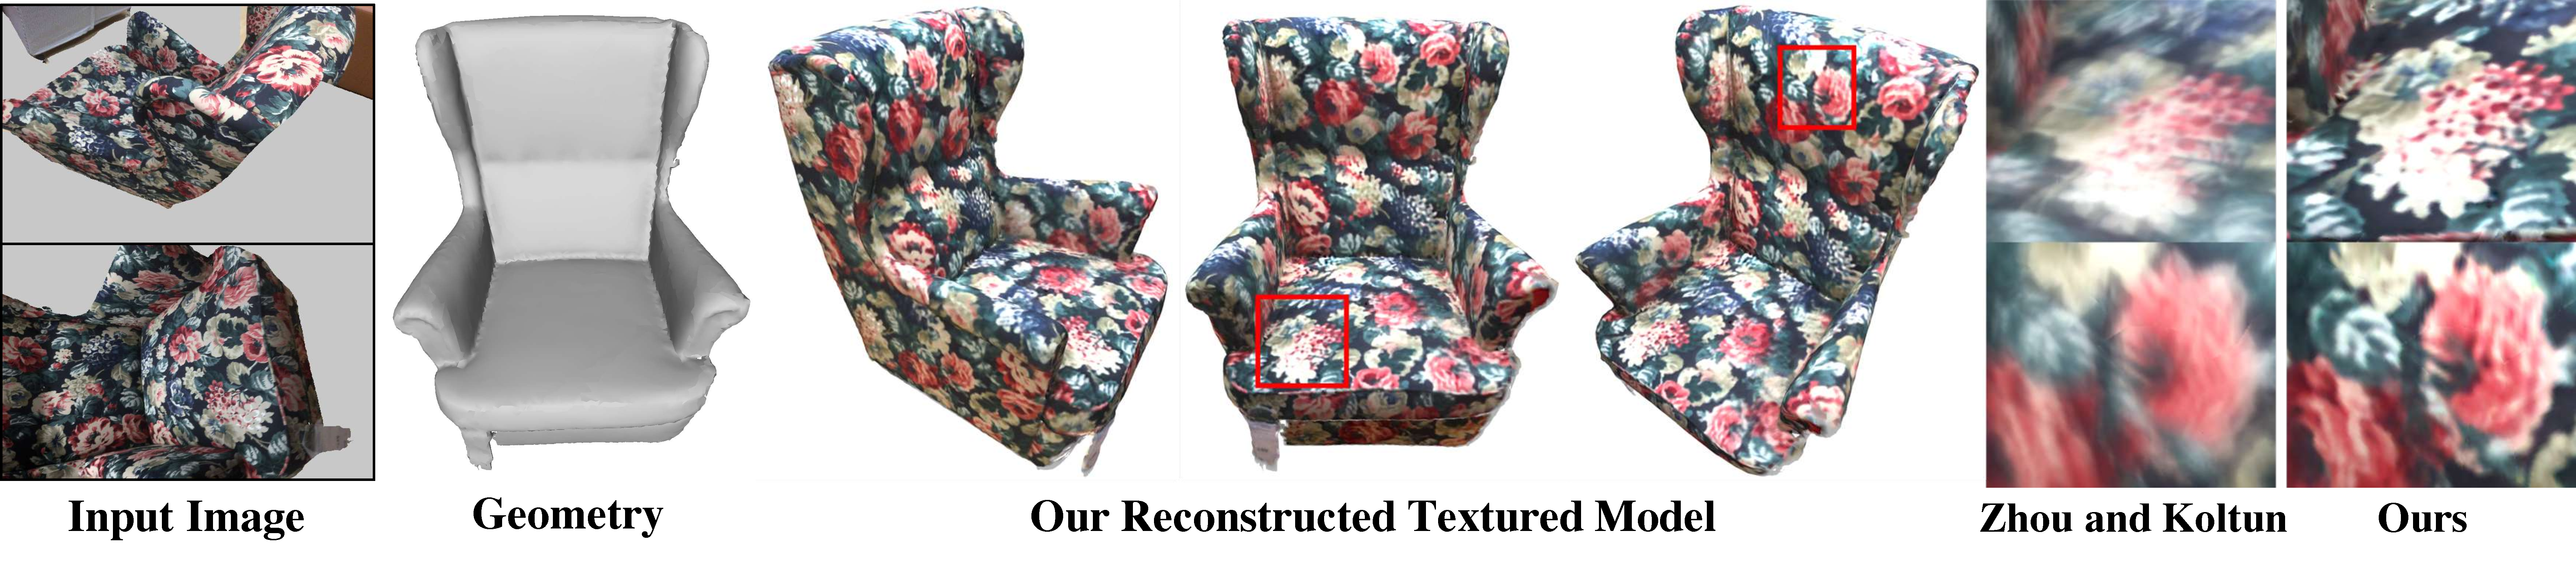
\includegraphics[width=\textwidth]{texturegen/figures/teaser-n.pdf}
    \caption{Our goal is to reconstruct high-quality textures from a 3D scan with aligned input images. Traditional methods optimize for a parametric color map to reduce misalignment error (Zhou and Koltun~\cite{zhou2014color}). We seek a better color consistency optimization and view aggregation method, and further derive a flexible texture optimization framework based on a learned metric that is robust to common scanning errors.}
    \label{fig:toptim-teaser}
\end{figure}

High-quality reconstruction is challenging for many reasons. The color quality of existing 3D reconstruction methods often suffers from artifacts due to motion blur and rolling shutter from commodity color cameras. 
This is compounded by oversmoothing and camera pose micro-misalignments due to popular reconstruction techniques.
For instance, the seminal volumetric fusion work~\cite{curless1996volumetric} is commonly used to generate a 3D model from input RGB-D frames by performing a weighted average over projected depth and color observations.
While effectively regularizing out noise, this also results in oversmoothed geometry and color.
Additionally, since camera poses are computed from imperfect color and noisy, relatively low-quality depth, they often suffer from micro-drift, which further exacerbates resulting visual artifacts such as ghosting and oversmoothing. To overcome these problems, various approaches have been developed to optimize color textures using models to adjust camera poses~\cite{zhou2014color}, distort images~\cite{bi2017patch,zhou2014color}, and balance colors \cite{zhou2014color}.  However, these prior approaches are not expressive enough and/or their optimization algorithms are not robust enough to handle the complex distortions and misalignment -- and therefore they fail to produce high-quality results for typical scans as shown in the results from Zhou and Koltun~\cite{zhou2014color} in Figure~\ref{fig:toptim-teaser}. We aim at designing novel methods to produce high-quality textures (Ours in Figure~\ref{fig:toptim-teaser}) from the noisy inputs including errors from geometry, images and camera poses.

\paragraph*{Methodology:} From the graphics perspective, we observe that the surface textures are more important to visual perception than geometry; for instance, many video games make use of techniques such as billboarding or bump mapping~\cite{decoret1999multi}
to achieve high-detail visuals at low cost, with an almost imperceptible difference to using accurate geometry. Therefore, accurate geometric reconstruction can be heavy and unnecessary, while light-weighted approximations of the scanning geometry with artifact-free primitives or CAD models are favored for interactive applications, including gaming and virtual/augmented reality. 
%
Thus, our first insight is to assume inaccurate geometries from scanning and focuses on high-quality texture reconstruction. While previous works suffer from optimizing camera poses to enhance geometry, we directly deliver ready-to-use geometries by approximating noisy scans with light-weight primitives or CAD models.
%
For large-scale indoor scenes, we abstract them with 3D planes by merging primitives detected from video frames, globally refine the planar structures, and complete the scene using the plane prior. For object-level scans, we simply replace them with CAD models and focus on the high-quality texture reconstruction under the misalignment between geometry and RGB images.

\begin{figure}
    \centering
    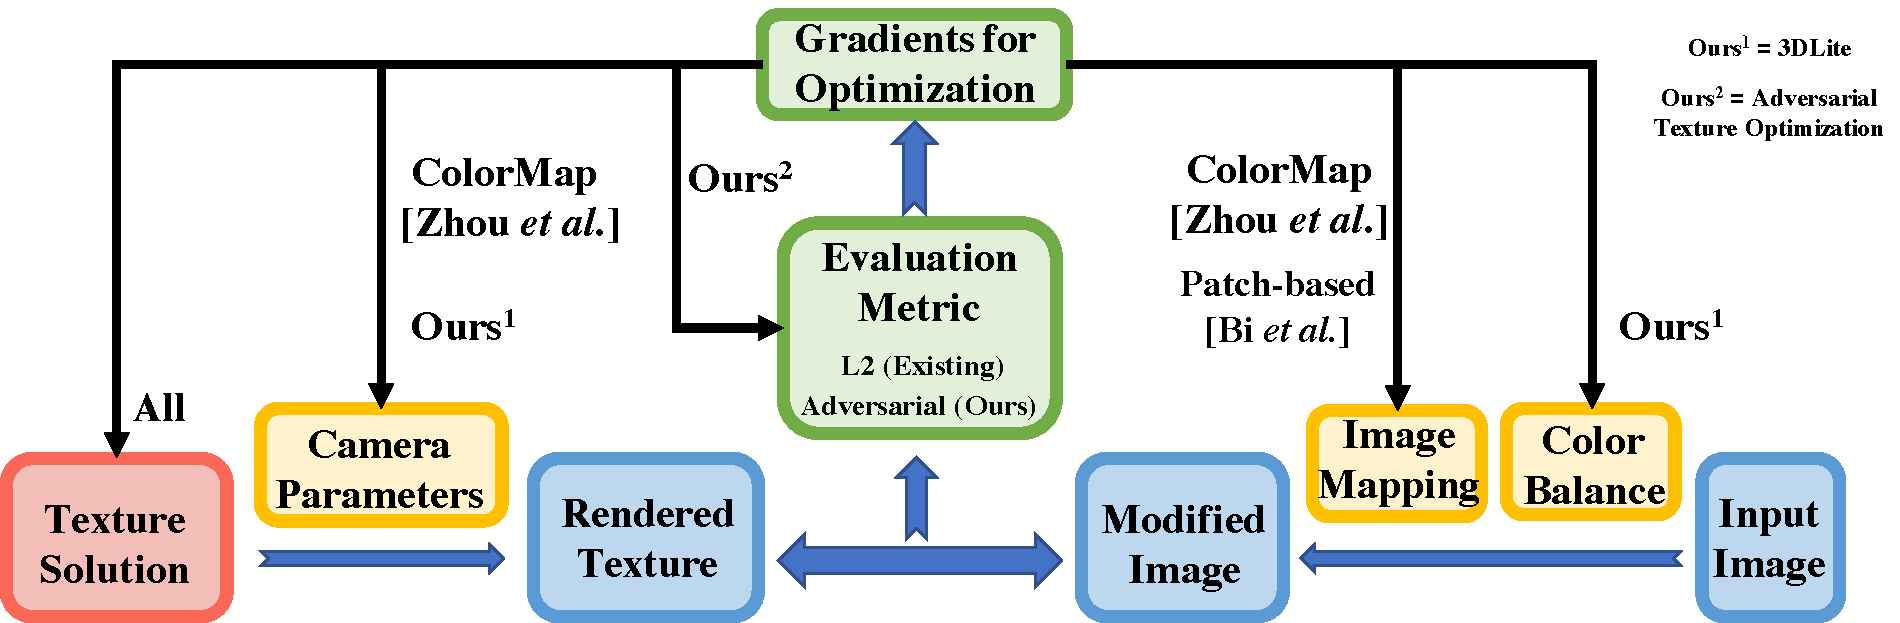
\includegraphics[width=\linewidth]{texturegen/figures/concept.pdf}
    \caption{All methods target at optimizing a texture solution based on a photo-consistency energy. Existing methods optimize the texture jointly with camera parameters~\cite{zhou2014color} or image mapping~\cite{zhou2014color,bi2017patch}. We adopt a powerful explicit parametric model and a robust optimization scheme in 3DLite~\cite{huang20173dlite}, or jointly solve texture with an adversarial evaluation metric in Adversarial Texture Optimization~\cite{huang2020adversarial}.}
    \label{fig:toptim-concept}
\end{figure}

To address the high-quality texture reconstruction problem under misalignment and errors, we abstract it as a general optimization problem as shown in Figure~\ref{fig:toptim-concept}.
%
We propose two different directions for improving texture optimization. In our first approach~\cite{huang20173dlite}, we employ a sparse-to-dense optimization, using sparse color features and geometric primitive constraints to help reach the basin of convergence of the L2 dense photo-consistency energy. We additionally incorporate color balance into our parametric model to make it more descriptive and optimize a sharp view selection to tackle the motion blur problem. Our second approach~\cite{huang2020adversarial} proposes a flexible texture optimization framework based on a learned metric that is robust to common scanning errors.
The key idea is to account for misalignment in a {\em learned objective function} of the texture optimization.   
Rather than using a traditional object function, like $L1$ or $L2$, we learn a new objective function (adversarial loss) that is robust to the types of misalignment present in the input data.  This novel approach eliminates the need for hand-crafted parametric models and replaces them all with a learned evaluation metric (green box in Figure~\ref{fig:toptim-concept}).  As such, it adapts to the input data and produces realistic texture reconstruction.

\paragraph*{Contribution:} By abstracting the complex scenes with structured primitives or objects with CAD models, we can produce lightweight, complete and artifact-free geometries from scans. Our texture reconstruction approaches demonstrate notably improved performance compared to state-of-the-art methods, both quantitatively on synthetic data and qualitatively on real data. This opens up the potential to produce CAD models with realistic textures. This feature enables realistic content creation for the gaming industry and virtual reality applications in the future, where nowadays 3D contents are still created by specialized artists with a huge amount of time and cost.

Although our methods are specifically designed for texture reconstruction, they can be further extended to address the general observation fusion problem, where we have several observed information of a unique system and want to merge the information. For example, we can collect various information taken from different viewpoints of the 3D geometry. Such information can be collected as physical properties using different sensors, or high-level semantics from the neural networks. All the information can be fused back to the geometry by extending either of our approaches. Our first approach highlights the importance of jointly optimizing the system under trusted sparse correspondences with dense consistency energy. With enough data supervision, our second approach exploits enable the automatic fusion with a learned metric, without designing hand-crafted fusion schemes.

\section{Surface Parameterization}
\label{intro:param}
This section discusses seamless surface parameterization as a necessary step towards texture understanding and formulates it as a quadrangulation problem. We will discuss the technical details for our quadrangulation method in Chapter~\ref{chapter:param}.

\paragraph*{Motivation:} For adversarial texture optimization~\cite{huang2020adversarial}, we apply the 2D convolution to learn a misalignment-tolerant metric in the image space.
%
A natural extension is to directly apply a CNN in the texture domain of a 3D surface.
%
The advantage of applying a CNN operator on 3D data over 2D images is obvious: it is relatively unaffected by view-dependent image effects, such as perspective, occlusion, lighting, and background clutter.
%
There have been a lot of recent works on the semantic segmentation of 3D data using 3D CNNs. However, the resolution of current 3D representations is generally quite low (2cm is typical), and so the ability of 3D CNNs to discriminate fine-scale semantic patterns is usually far below their color image counterparts \cite{long2015fully,he2017mask}.
%
Fortunately, texture signals lie on the surface instead of the whole 3D volume. This opens the opportunity for us to parameterize the surface using a 2D domain and apply a 2D convolution in the parameterization space. We observe the key difference between 2D images and 3D surfaces is that the image coordinate system serves as a consistent global definition of how the 2D domain is parameterized, while there is no global consistent definition of surface parameterization in 3D. For example,
 \begin{figure}
    \centering
     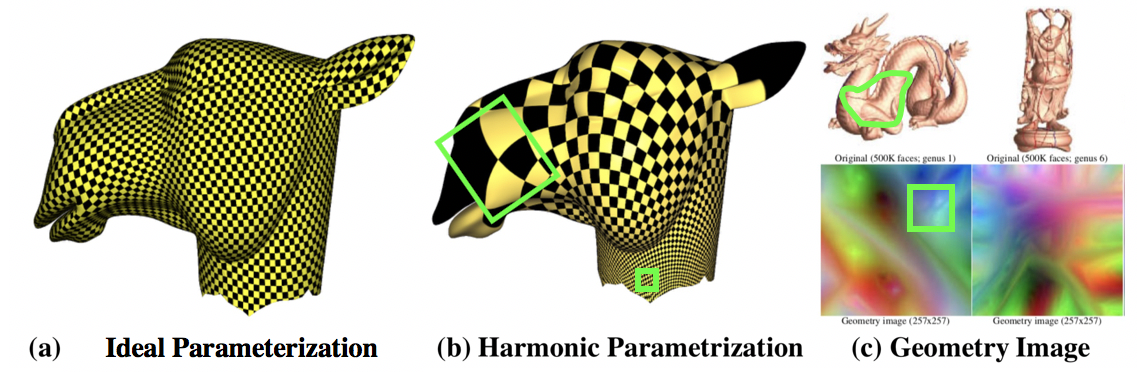
\includegraphics[width=0.8\linewidth]{quadriflow/param.png}
     \caption{(a) With an ideal parameterization, we can get the surface parameterization aligned with shape features with negligible distortion. (b) Harmonic parameterization leads to high distortion in the scale. (c) Geometry images~\cite{gu2002geometry} result in high distortion in the orientation.}
     \label{fig:intro-quadriflow-param}
 \end{figure}
different existing parameterization methods have different problems as shown in Figure~\ref{fig:intro-quadriflow-param}, where the receptive field of the convolution (marked as green edges) can have significant different scales with harmonic parameterization or irregular neighborhoods with geometry images~\cite{gu2002geometry}. An ideal parameterization for convolution should be regular, uniform and seamlessly connected. In this case, the receptive field is regular and canonicalized with the same shape and size. Such a parameterization is shown in Figure~\ref{fig:intro-quadriflow-param}(a), where the surface is seamlessly parameterized and looks like a uniform-scale quadrilateral mesh. Therefore, to tackle the texture convolution problem, we need to build a robust and scalable quadrangulation to convert a general triangle mesh as a uniform-scale and regular quadrilateral mesh.

\paragraph*{Methodology:} State-of-the-art quadrangulation method~\cite{bommes2009mixed} casts the problem of seamless global parametrization as a mixed-integer constrained optimization problem (MIP), which is slow and it does not scale well to large meshes. The much more efficient Instant Meshes algorithm of Jakob et al.~\cite{jakob2015instant} uses local smoothing operators to compute an orientation field and a position field quickly. However, it produces many singularities in the position field as irregular vertices. Unfortunately, irregular vertices can cause problems for applications; for instance, they cause unsightly visual artifacts in Catmull--Clark subdivision, or additional work for an artist to edit a model. In our texture understanding scenario, such irregularity means that our convolution kernels are highly distorted or not canonically oriented near the singularity positions.
%
We present \emph{QuadriFlow}~\cite{huang2018quadriflow}, a scalable, robust algorithm for automatic quad meshing that builds upon Instant Meshes but uses a global method to remove all the singularities from the position field.
We reformulate the quadrangulation problem as continuous objective energy from Instant Meshes with a set of constraints of integer variables to remove position-field singularities. We optimize the continuous energy and adjust integer variables to satisfy the constraints in two separate stages. The second stage is simplified as an integer linear programming problem, and we further approximate it by a minimum cost network flow problem for which a solution is guaranteed to be found in polynomial time. Thus, our method removes all singularities in the position field and robustly produces a regular quadrilateral mesh.

\paragraph*{Contribution:} We formulate the quadrangulation problem as a MIP problem, and apply several levels of approximations where a global optimum can be found with an efficient solution. Therefore, we obtain a robust and scalable algorithm that can handle meshes with millions of faces. Since the global optimum is guaranteed, our method produces even better mesh qualities compared to results from MIP solver according to the mesh distortion or edge length variance. Since our problem is theoretically feasible, we guarantee to remove all singularities from the position field. We process a one-million triangle mesh in five seconds, while MIP solver can only handle thousands of triangles in ten minutes.
%
Our algorithm is beneficial to many problems in the geometry processing community since quadrilateral meshes are particularly useful for Catmull--Clark subdivision surfaces, texturing, mesh editing, visualization, and physics-based simulation. For example, our implementation has been integrated to non-commercial or commercial geometry software including BakeMyScan\footnote{\url{http://bakemyscan.org}} for texturing and Dynremesh\footnote{\url{https://blendermarket.com/products/dynremesh-2}} for mesh editing.
%
In addition, our method is not only specifically valuable for quadrangulation. Since we generally approximate a mixed-integer programming problem, our method can be used for real problems with similar mathematical formulations in industrial productions, including job-shop modeling. One important example that happens in agricultural production planning involves determining production yield for several crops that can share resources (e.g. Land, labor, capital, seeds, fertilizer, etc.)\footnote{\url{https://en.wikipedia.org/wiki/Integer_programming}}.
%
Finally, our algorithm provides robust and efficient computation for regular and seamless surface parameterization, which is the basis for texture understanding task which we will discuss in the next section.

\section{Texture Understanding}
\label{intro:understand}
\begin{comment}
With the surface parameterization, we propose a surface convolution operator that extracts effective features in the parameterization space (Section~\ref{intro:texture-learn}).
%
Specifically, we apply the proposed convolution operator in a well-defined geodesic neighborhood where each point is locally parameterized with a 2D coordinate based on our seamless parameterization.
%
We make our novel convolution operator four-way rotationally symmetric to canonicalize the feature extraction so as to address the existence of orientation ambiguities in the parameterization.
%
Our surface convolution is a 2D operator that effectively handles, and thereby outperforms other less efficient dense 3D convolution operators.
%
We find that the surface parameterization serves not only as a basis for surface convolution operators but also as useful information that is highly correlated with the color signals. Therefore, we create a dataset with pairs of RGB images and pre-computed 3D canonical frames from the scanning data and train a neural network to predict frames from color signals. Our network improves low-level vision tasks including surface normal estimation and feature matching, thus enabling high-level applications in augmented reality (Section~\ref{intro:frame}).
\end{comment}


Given our seamless parameterization of the surface, we are able to explore the texture understanding problem. This section introduces two significant developments: the semantic 3D scene understanding problem using parameterized textures, as well as the 3D frame understanding problem given  RGB images. We discuss more technical details in Chapter~\ref{chapter:texturenet}.

\vspace*{10pt}\noindent We first present the 3D scene understanding problem.

\paragraph*{Semantics from Texture.}
\begin{figure}
    \begin{center}
        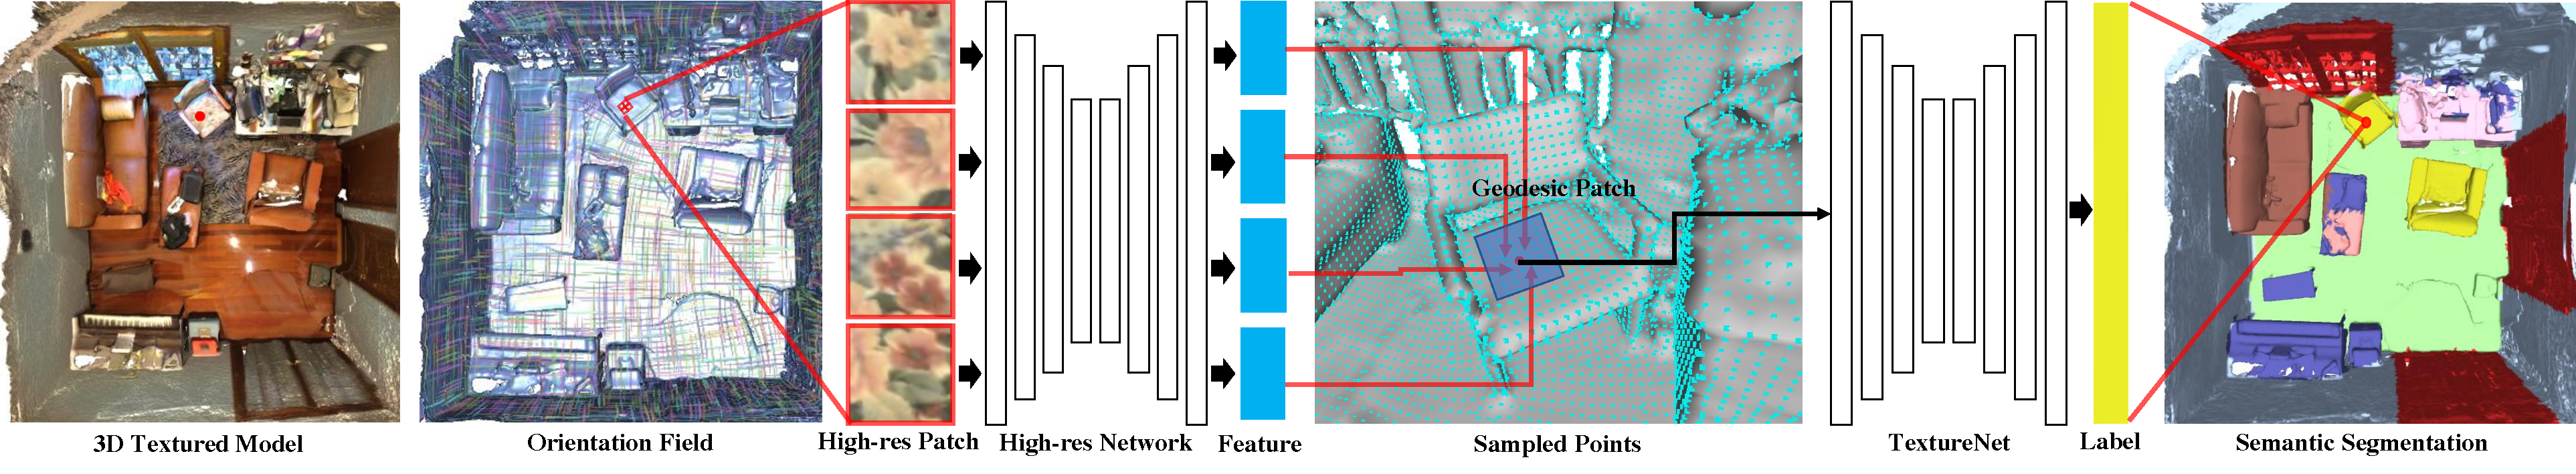
\includegraphics[width=\linewidth]{texturenet/teaser/teaser.pdf}
        \caption{TextureNet takes as input a 3D textured mesh.  The mesh is parameterized with a consistent 4-way rotationally symmetric (4-RoSy) field, which is used to extract oriented patches from the texture at a set of sample points.   Networks of 4-RoSy convolutional operators extract features from the patches and used for 3D semantic segmentation.}
        \label{fig:texturenet-teaser}
    \end{center}    
\end{figure}
\label{intro:texture-learn}

\paragraph*{Motivation:} 3D semantic segmentation is a fundamental task for 3D understanding. There has been a lot of recent work on the semantic segmentation of 3D data using convolutional neural networks (CNNs).  Typically, features extracted from the scanned inputs (e.g., positions, normals, height above ground, colors, etc.) are projected onto a coarse sampling of 3D locations, and then a network of 3D convolutional filters is trained to extract features for semantic classification -- e.g., using convolutions over voxels \cite{wu20153d,maturana2015voxnet,qi2016volumetric,song2017semantic,dai2017scannet,dai2018scancomplete}, octrees \cite{riegler2017octnet}, point clouds \cite{qi2017pointnet,qi2017pointnet++}, or mesh vertices \cite{masci2015geodesic}.  The advantage of these approaches over 2D image-based methods is that convolutions operate directly on 3D data, and thus are relatively unaffected by view-dependent image effects, such as perspective, occlusion, lighting, and background clutter.   However, the resolution of current 3D representations is generally quite low (2cm is typical), and so the ability of 3D CNNs to discriminate fine-scale semantic patterns is usually far below their color image counterparts \cite{long2015fully,he2017mask}. Given our robust seamless surface parameterization, we have the opportunity to apply our convolutions in the 2D parameterization space and thereby extract view-independent and high-resolution features.

\paragraph*{Methodology:} We propose a new convolutional neural network, \emph{TextureNet}~\cite{huang2018texturenet}, with a 2D convolution kernel that extracts features directly from high-resolution signals associated with 3D surface meshes.  Given our surface parameterization, we locally unwrap the geometry into a regular 2D square where we apply a 2D convolution. There is a 4-way orientation ambiguity in our surface parameterization, and we accordingly introduce a new convolutional operator invariant to such ambiguity called texture convolution. Our network can be viewed as a UNet~\cite{ronneberger2015u} architecture composed of our texture convolution.

\paragraph*{Constribution:} As an example application, we demonstrate the benefits of our architecture for 3D semantic segmentation of textured 3D meshes (Figure~\ref{fig:texturenet-teaser}).  The results show that our method outperforms all existing methods on the basis of mean IoU by a significant margin in both geometry-only (6.4\%) and RGB+Geometry (6.9-8.2\%) settings. Further, our texture convolution is a general local descriptor that can be used for other learning tasks. Since our kernel is intrinsically aligned with the shape feature given the surface parameterization, it is potentially effective for many tasks that require intrinsic features, including human body segmentation~\cite{maron2017convolutional} and non-rigid registration~\cite{litany2017deep}.

\vspace*{10pt}\noindent We now proceed to the 3D frame understanding problem form a single image.

\paragraph*{Canonical Frame Understanding from RGB Images.}
\label{intro:frame}

 \begin{figure}
    \centering
    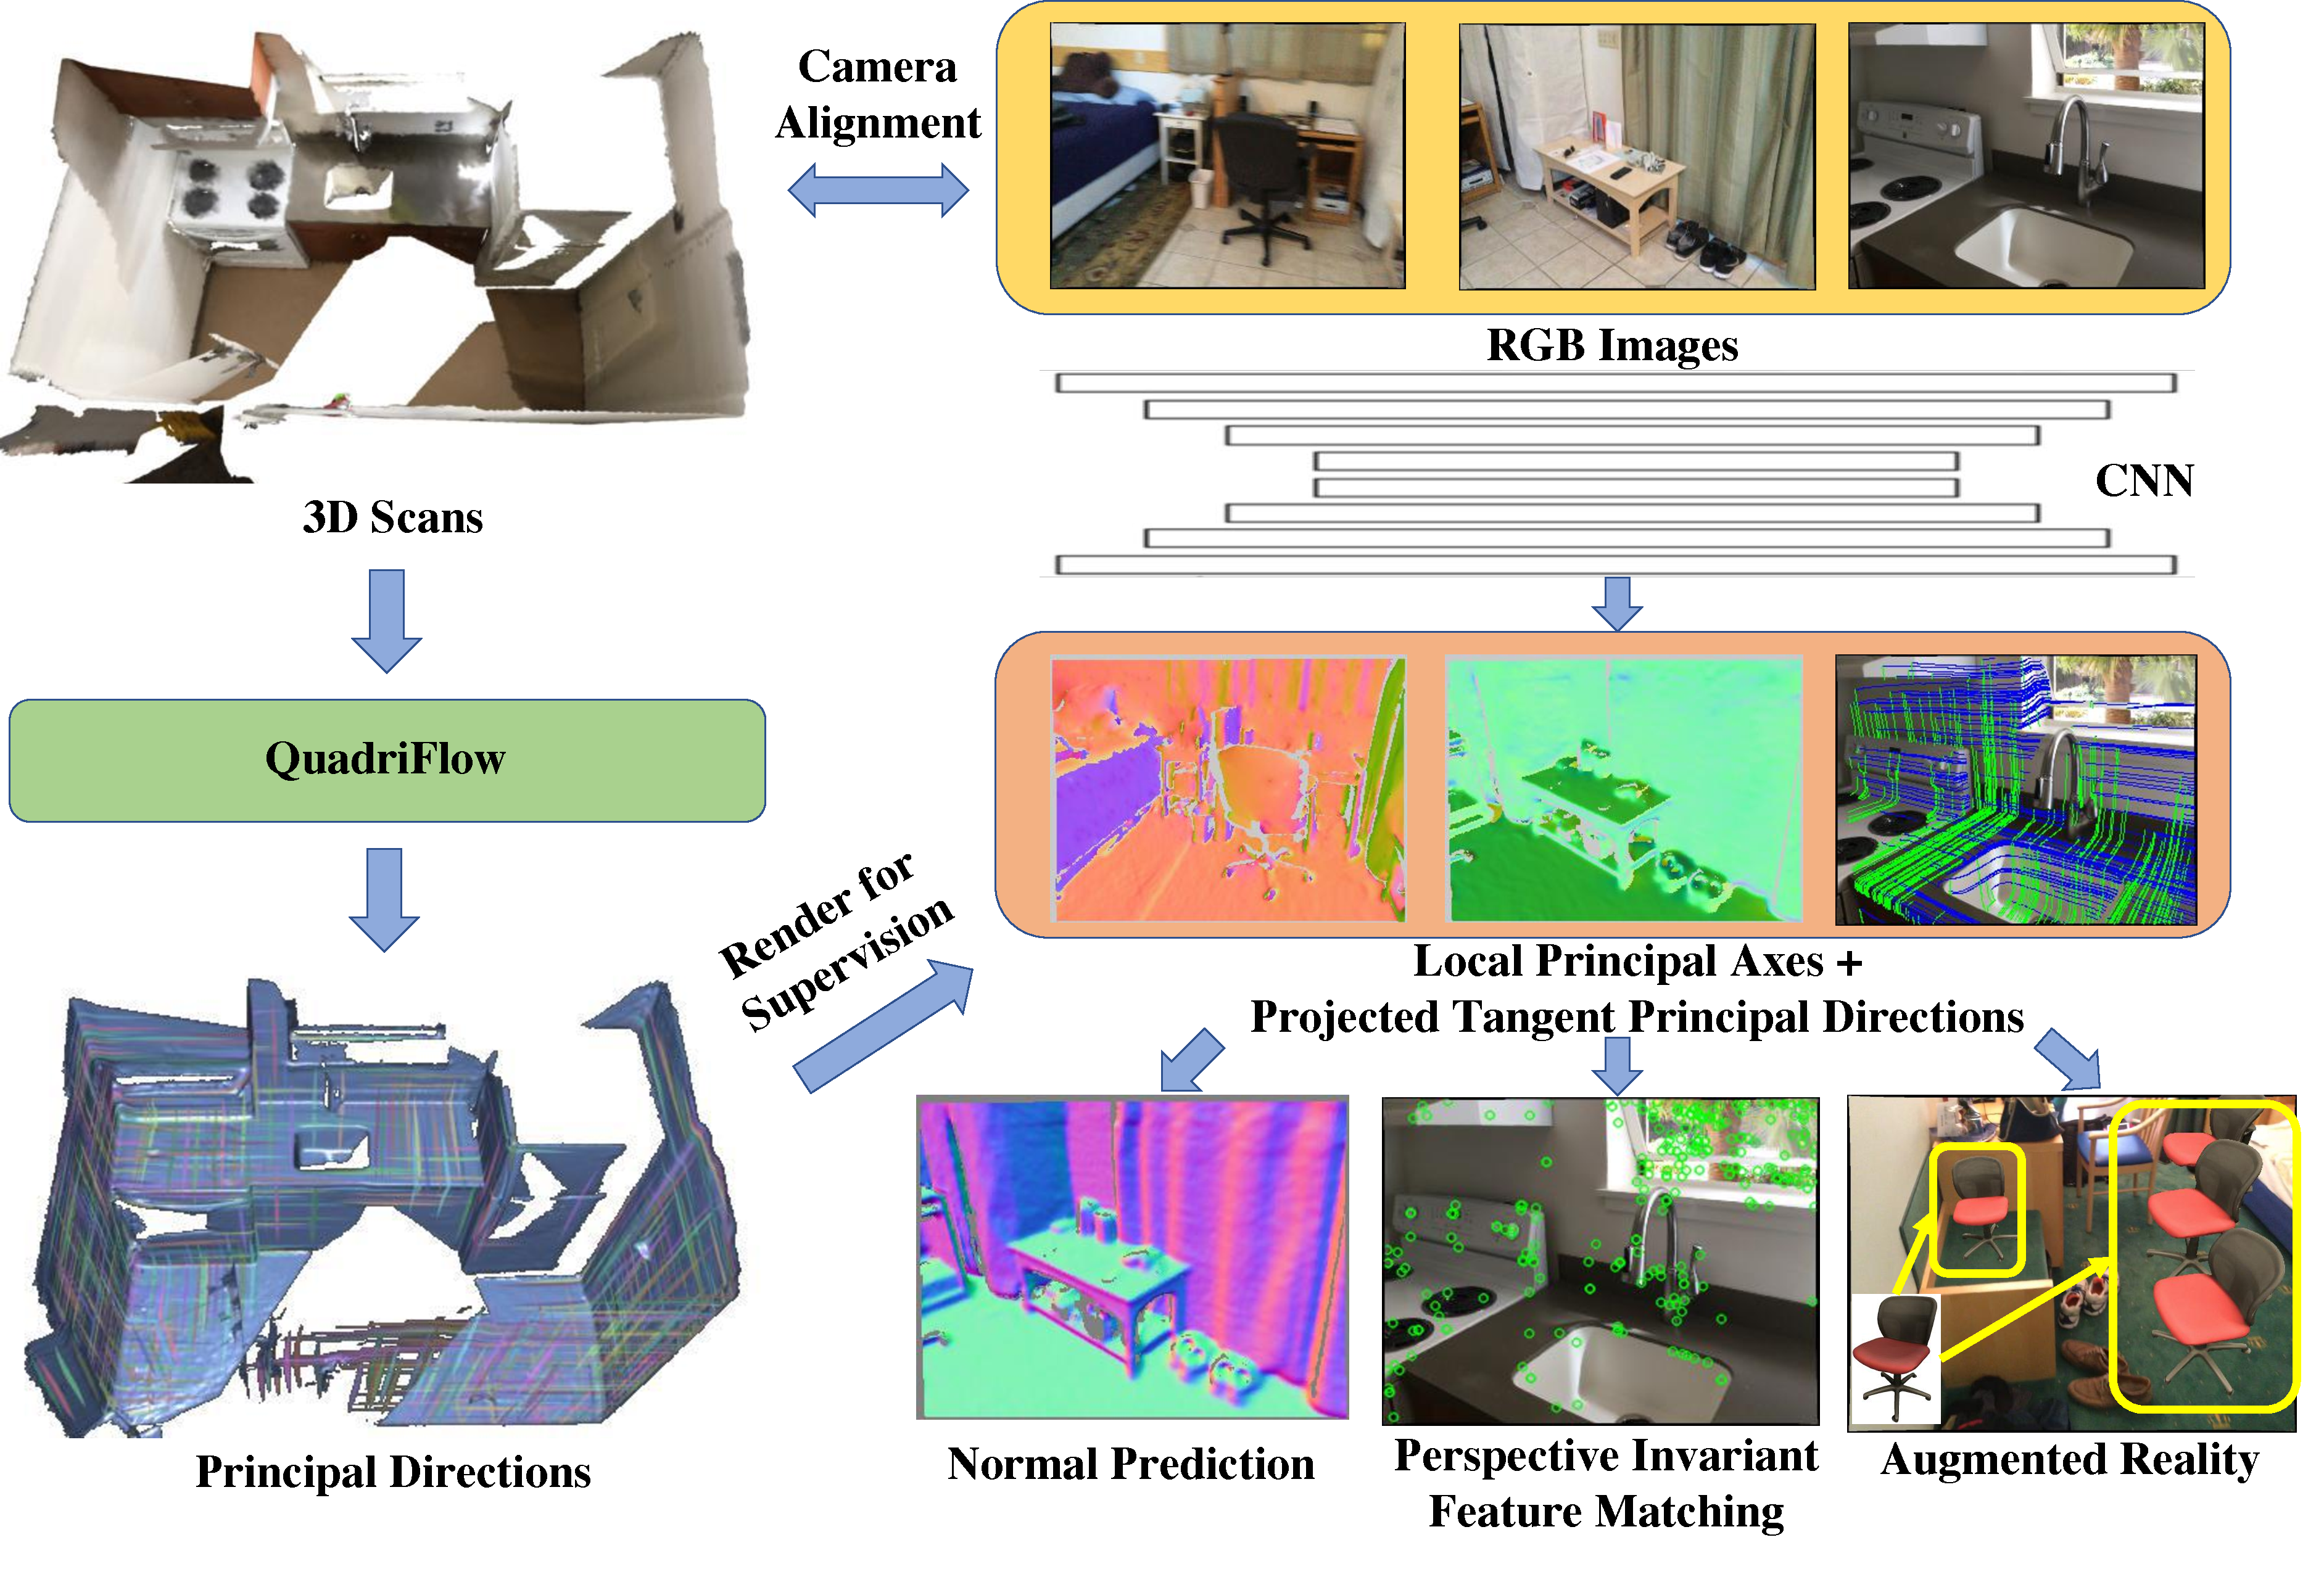
\includegraphics[width=0.75\linewidth]{FrameNet/graph/teaser.pdf}
    \caption{We propose the novel task of predicting dense 3D \cframe{} from a single RGB image. We compute the frames from reconstructed meshes using QuadriFlow and render them to images to supervise the task.  We train a network that predicts all directions of the frames jointly.  We find that predicted tangents provides better surface normals, and are useful for applications like feature matching and augmented reality.}
    \label{fig:framenet-teaser}
    \vspace{-0.1in}
\end{figure}

\paragraph*{Motivation:} In recent years, learning to predict 3D properties from a single RGB image has made great progress.  For example, monocular depth estimation~\cite{shelhamer2015scene,li2017two,xu2017multi,wang2018adaptive,fu2018deep} and surface normal prediction~\cite{eigen2015predicting,wang2015designing,bansal2016marr,qi2018geonet} have improved dramatically.  There are many applications for these tasks in scene understanding and robot interaction. 
%
The main challenge in this domain is choosing an appropriate representation of 3D geometry to predict.  Zhang~\textit{et al.}~\cite{zhang2018deep} predict dense surface normals and then use geometric constraints to solve for depth with global optimization.  GeoNet~\cite{qi2018geonet} predicts both surface normals and depth and then passes them to a refinement network for further optimization.  These methods are clever in their use of geometric constraints to regularize dense predictions.   However, they infer only 2 of the 3 degrees of freedom in a 3D coordinate frame -- the rotation in the tangent plane around the surface normal is left unknown.  As such, they are missing 3D information critical to many applications.  For example, they cannot assist an AR system in placing a picture frame on a wall or a laptop on a table because they don't know the full 3D coordinate frame (including tangent directions) of the wall or table surfaces.

\paragraph*{Methodology:} With our canonical surface parameterization, such 3D coordinate frames can be easily acquired given the geometry. Therefore, we propose a novel image-to-3D task: dense 3D \cframe{} estimation from a single image (figure~\ref{fig:framenet-teaser}).  This task requires predicting a full 3D coordinate frame defined by the surface normal {\em and two principal tangent directions} of the surface observed at every pixel in an RGB image.  We train a neural network for this task in a supervised setting given pairs of RGB and canonical frame images.   To acquire ``ground truth'' \cframe{}, we leverage data from RGB-D scanning datasets, like ScanNet~\cite{dai2017scannet}, which provide large sets of images posed within reconstructed 3D meshes.  
We compute \cframe{} on the meshes and render them to the RGB images to produce training data. The full pipeline is shown in Figure~\ref{fig:framenet-teaser}.

\paragraph*{Constribution:} This novel task is beneficial to both low-level and high-level tasks and applications.  First, we find that predicting principal tangent directions is easier than predicting normals because they are often aligned with observable patterns in surface textures (e.g., wood grains, fabric weaves, tile seams, etc.) and surface boundaries, which are directly observable in images.  Second, Joint surface normal and tangent prediction is more robust than normal prediction alone due to the regularization provided by orthogonality constraints. Therefore, our method outperforms the direct surface normal estimation methods.  Third, With a full canonical 3D coordinate frame estimation at every pixel, we are able to transform the local patch into the canonical tangent space where local patch descriptors like SIFT~\cite{lowe2004distinctive} are perspective invariant and robust for correspondence matching. A particularly compelling application of predicting 3D surface frames is augmented reality -- i.e., it enables adding new elements to a scene with appropriate 3D orientations.

\section{Contribution Summary}
\label{intro:contribution}

\begin{figure}
    \centering
    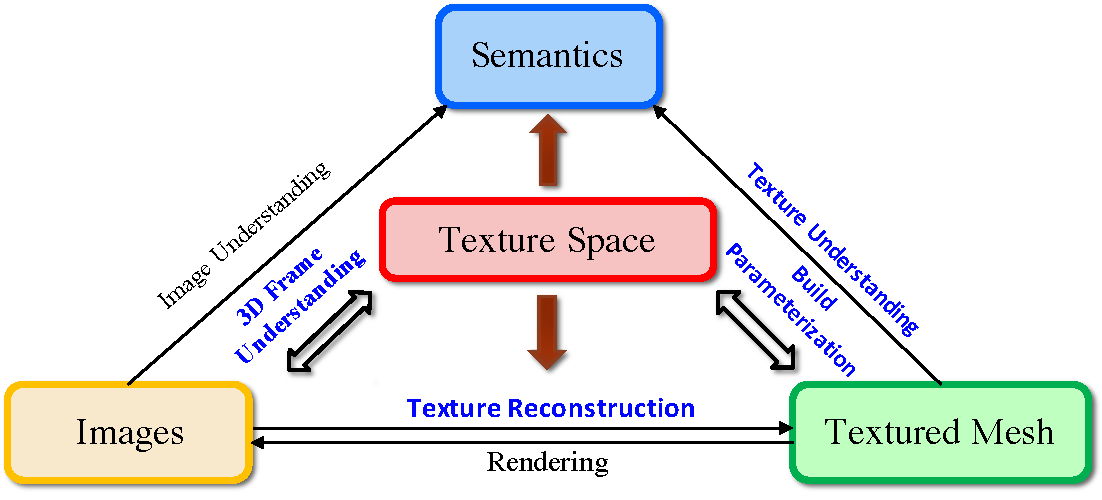
\includegraphics[width=0.75\linewidth]{intro/concept.pdf}
    \caption{Surface texture processing is related to four components. Images and textured mesh can be converted to each other via reconstruction and rendering. Semantics can be inferred from both of them. The surface parameterization can build a map between the texture space and the surface. Semantics can be effectively learned with convolutions in the texture space, which can be inferred from color signals.}
    \label{fig:intro-concept}
\end{figure}

As described above, this thesis addresses surface texture processing and its applications. Figure~\ref{fig:intro-concept} summarizes the main components related to our surface processing problems, where we specifically solve the tasks with names rendered in blue. Basically, surface texture and the scanned images can be converted to each other via rendering and reconstruction. We focus on reconstructing high-quality surface texture from images. We propose to construct a texture space using our new seamless surface parameterization. This leads to an important representation that is helpful for texture understanding. including semantics scene understanding from parameterized textures and canonical frame inference from images.

Overall, the contributions of this thesis include:
\begin{itemize}
    \item We address the surface texture reconstruction problem, propose a novel parametrization of the texture space, and show its usefulness in texture understanding.
    \item We propose \emph{3DLite}, an approach to produce high-quality surface textures on top of lightweight planar geometry abstracted from the scan.
    \item We propose an \emph{adversarial texture optimization} method to produce photorealistic textures for approximate surfaces, even from misaligned images, by learning an objective function that is robust to scanning errors.
    \item We propose \emph{Quadriflow}, a scalable and robust quadrangulation algorithm that is solvable in polynomial time.
    \item We design \emph{TextureNet} as a novel neural network for extracting features from high-resolution signals living on surfaces embedded in 3D. 
    \item We observe the high correlation between surface parameterization from \emph{Quadriflow} and RGB signals on surface texture, and identify an important new 3D vision problem with a solution called \emph{FrameNet}: local canonical frame estimation from RGB images.
\end{itemize}

While image processing and geometry processing are both classical and well-established fields, the processing of image data living on surfaces, surface textures, has not received the attention it deserves. This thesis makes a number of fundamental contributions to the new area of surface texture processing and it is our hope that it will motivate further efforts and progress in the area. 

%%%%%%%%%%%%%%%%%%%%%%%%%%%%%%%%%%%%%%%%%%%%%%%%%%%%%%%%%%%%%%%%%%%%%
\begin{comment}
The 3D environment is digitally represented as a textured mesh, including geometry and color information. The geometry information is contained in the triangle mesh with a set of vertices and triangles connecting them. Since color is associated with the surface, it is represented as the surface texture with a UV parameterization and a texture image. First, we associate an additional 2D coordinate with each vertex so that each 3D region is mapped to a 2D parameterization space. The association of the 2D coordinate is called the UV parameterization, and the 2D space is named as the UV space in the computer graphics community. A texture image is used to store the color in the UV space so that the surface color can be determined by sampling through the mapping. Figure~\ref{fig:intro-texture-represent} illustrates how the textured mesh is represented in the computer.
\begin{figure}
    \centering
    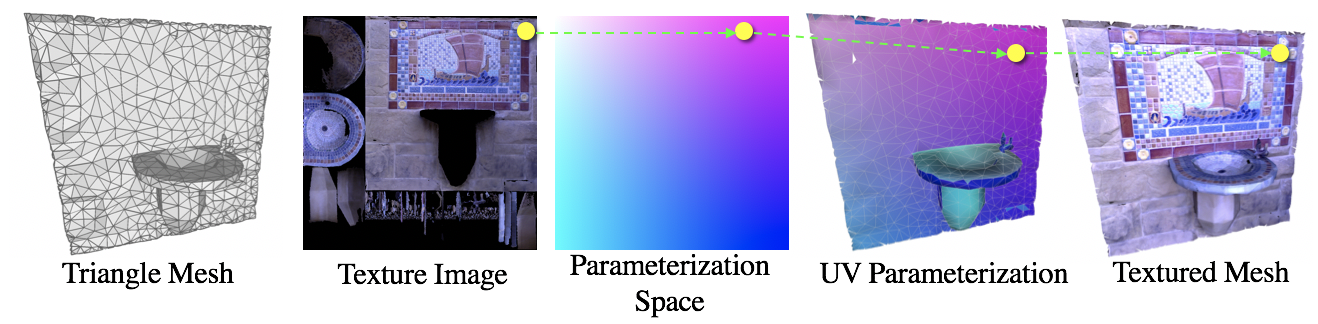
\includegraphics[width=\linewidth]{intro/texture-represent.png}
    \caption{Textured mesh representation in the computer. The geometry information is stored as a triangle mesh. The color information is stored as a surface texture with a UV parameterization for all vertices and a texture image stored in the parameterization space.}
    \label{fig:intro-texture-represent}
\end{figure}
We focus on the surface texture processing -- reconstructing and understanding the surface texture based on commodity RGB-D cameras.
\end{comment}

\begin{comment}
By reconstruction, we aim to produce high-quality texture from inaccurate and low-quality scanning data.  However, producing a photorealistic textured mesh of real-world environments requires not only geometric reconstruction but also high-quality color reconstruction.
Unfortunately, due to noisy input data, poorly estimated surface geometry, misaligned camera parameters, unmodeled optical distortions, and view-dependent lighting effects,  aggregating multiple real-world images into high-quality, realistic surface textures is still a challenging problem. We aim at addressing this problem by minimizing color inconsistency or jointly optimizing the texture with a learned metric, as described in Section~\ref{intro:texture-recon}.
\end{comment}

\begin{comment}
While our deep metric can be implemented with an image convolutional neural network (CNN) as a widely-studied deep learning technique, one extension in this thesis is to directly apply a CNN in the texture domain of the 3D surface.
%
The advantage of applying a CNN operator on 3D data over 2D images is obvious: convolutions directly applied to 3D data are relatively unaffected by view-dependent image effects, such as perspective, occlusion, lighting, and background clutter.
%
There has been a lot of recent works on semantic segmentation of 3D data using 3D CNNs. However, the resolution of current 3D representations is generally quite low (2cm is typical), and so the ability of 3D CNNs to discriminate fine-scale semantic patterns is usually far below their color image counterparts \cite{long2015fully,he2017mask}.
%
We believe a 2D CNN applied in the texture domain of the 3D surface can address the above issue, and the key challenge is to obtain a consistent and canonical surface parameterization that maps the 3D surface into a 2D space where 2D convolutions can be applied.
%
We find that this challenge is related to the seamless surface parameterization problem in the computational geometry community. While this problem has been studied for more than a decade, existing methods formulated it as a mixed-integer programming problem (NP-hard), where an effective and robust solution is unavailable.
%
We reformulate the problem and obtain a robust and efficient seamless parameterization of the geometry of a complex 3D environment (Section~\ref{intro:param}).
\end{comment}

\begin{comment}
 \begin{figure}
  \centering
  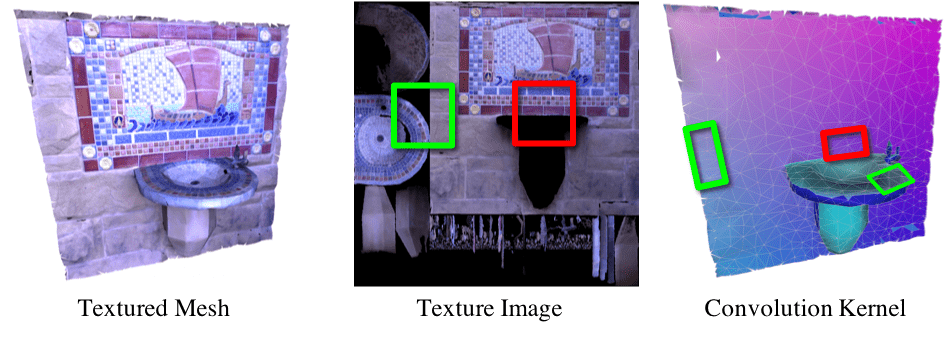
\includegraphics[width=0.8\linewidth]{intro/uvconv.png}
  \caption{Limitation of convolutions with a general UV parameterization. The convolution applied to the texture image incorrectly aggregates disconnected regions (green) and incorporates unexpected boundaries (red).}
  \label{fig:intro-uv-param}
\end{figure}
For example, the most straightforward idea is to directly use general UV parameterization. However, convolution applied to the texture image suffers can cause problems by breaking the connectivity information in the 3D. As shown in Figure~\ref{fig:intro-uv-param}, the green convolution kernel incorrectly aggregates disconnected regions of the mesh. Additionally, the red convolution kernel in the texture image reaches the boundaries, while ideally, this should not happen since the center is far from the surface boundary.
\end{comment}

